\chapter{Fazit}
Im Folgenden werden die Erkenntnisse der vorliegenden Arbeit zusammengefasst sowie die Fragen von RQ1 und RQ2
beantwortet. Abschließend wird das Ergebnis und das wissenschaftliche Vorgehen dieser Arbeit kritisch gewürdigt sowie Anregungen für 
weitere Forschungen in Folgearbeiten gegeben werden. 
\section{Zusammenfassung}

Im Allgemeinen haben Lernende als Schüler, Studierende oder sich Fortbildene Motivationsprobleme 
beim Lernen. Gerade im E-Learning ist die Fähigkeit zur Selbststeuerung des Lernprozesses besonders wichtig,
um einen positiven Lernerfolg zu haben. Dennoch fehlt es oft an der Kompetenz, selbständig und 
eigenmotiviert diesen Lernprozess zu gestalten.
CAs können als Ansprechpartner für die Gestaltung des Lernprozesses dienen.
Für einen optimalen Aufbau des Lernprozesses spielen charakteristische Merkmale wie der
Lernstil des Lernenden eine wichtige Rolle. Daher wurde in dieser Arbeit
die Machbarkeit analysiert, ob sowohl durch eine dialogbasierte Interaktion als auch durch ein Quiz-Spiel zwischen einem CA 
und einem Lernenden in natürlicher Sprache der Lernstil des Lernenden klassifiziert werden kann.
Zudem wurde untersucht, inwiefern die Interaktion mit einem CA für den Lernenden motivierend erscheint.
Das Vorgehen dieser Arbeit orientiert sich an die DSR Methodologie nach Hevner (2007).

Im ersten Schritt wurden mithilfe einer unsystematischen Literaturanalyse unterschiedliche Modelle von Lerntypologien
aufgestellt. In einem weiteren Schritt wurden die ausgewählte Lerntypologie des Lernstils und das Modell 
von Felder und Silverman (1988) sowie das ILS-Instrument durch eine Analyse der unterschiedlichen Modelle der Lerntypologien begründet dargestellt.
Der Prototyp namens Vicky kann den Lernstil des Lernenden auf zwei Arten bestimmen.
Zuerst führt Vicky einen Dialog mit dem Lernenden, wobei 17 Fragen des ILS-Fragebogens gestellt werden.
Anhand der Antworten des Lernenden wird im Hintergrund der Lernstil berechnet. In einer weiteren Interaktion
kann der Lernende zwischen einem vier oder acht Fragenquiz wählen. Anhand der Hilfestellungen, die Vicky während 
der Quiz-Frage anbietet, wird der Lernstil bestimmt. Für die Beantwortung der zwei wesentlichen Fragestellungen 
dieser Arbeit wurde eine Online-Umfrage (n=25) durchgeführt. Bei der Online-Umfrage haben die Probanden beide 
Interaktionen mit Vicky durchgeführt. Sie wurden zur Wahrnehmung von Vicky, zur Einschätzung der Lernstilklassifikation 
von Vicky und zur Beeinflussung auf die Lernmotivation befragt.

\textbf{RQ1:} \textit{\glqq Inwiefern ist es möglich, durch eine dialogbasierte Interaktion eines Lernenden in natürlicher Sprache mit einem persönlichen CA den individuellen Lernstil für den Lernenden zu bestimmen?\grqq{}} 

Für die Bestimmung eines individuellen Lernstils des Lernenden durch einen CA wurde ein Prototyp 
erstellt, welcher in Kapitel \ref{VorstellungPrototyp} ausführlich beschrieben wurde. Dieser bildet ein 
Level-1-Artefakt, welches als Interaktionsmedium in der Online-Umfrage
benutzt wurde. Der Theorieteil stellt 
zum einen das verwendete Lernstilmodell (vgl. Kapitel \ref{ATL}), welches die Basis des Prototyps darstellt,
und zum anderen die Funktionsweise des NLP sowie die positive Beeinflussung des Maschinellen Lernens
auf die natürliche Sprache, wodurch eine Interaktion per Chatgespräch ermöglicht wird, vor. 
Die Ergebnisse der Umfrage (vgl. Kapitel \ref{Kapitel5.2}) dienen der Beantwortung
von RQ1 und RQ2 dieser Arbeit.

Für die Machbarkeit einer Bestimmung eines individuellen Lernstils für den Lernenden mithilfe eines CAs
durch eine dialogbasierte Interaktion ergab die Umfrage ein positives Ergebnis. Vicky tendierte dazu, 
den individuellen Lernstil der Teilnehmer richtig einzuschätzen. 24 von 25 Probanden fühlten sich 
richtig eingeschätzt und waren mit der individuellen Klassifikation zufrieden, da diese als realistisch empfunden wurde.
Vicky wurde positiv bezüglich der Transparenz, der eleganten Antworten und der Verlässlichkeit bewertet. Dies könnte dazu
beigetragen haben, eine höhere Glaubwürdigkeit gegenüber der Akzeptanz des individuellen klassifizierten Lernstils zu
bewirken.

Die Bewertung des identifizierten individuellen Lernstils der Befragten durch das Quiz-Spiel fiel im Vergleich zur ersten 
Interaktion schlechter aus. Außerdem zeigten beide Interaktionsformen eine unterschiedliche Häufigkeit in den 
klassifizierten Lernstildimensionen auf.
Die größten Unterschiede wiesen der sensorische, visuelle, verbale und sequentielle Lernstil auf.
Ein möglicher Grund für diese Unterschiede könnte der Einfluss der Quiz-Fragen auf die Befragten darstellen,
sodass beispielsweise eine Hilfestellung gewählt wurde, die sich besonders eignet, um die Quiz-Fragen besser beantworten zu können,
obwohl der Proband generell einen anderen Lernstil präferiert. Ein weiterer Grund könnte die Verwendung des 
\glqq Solution-Buttons\grqq{} sein, wodurch die Klassifikation des Lernstils für die gestellte Frage entfällt.

\textbf{RQ2:} \textit{\glqq Inwiefern kann das Motivationsverhalten des Lernenden durch die Interaktion mit einem CA beeinflusst werden?\grqq{}}

Zur Messung des Einflusses auf das Motivationsverhalten der Befragten wurde das ARCS-Modell verwendet.
Bis auf die Dimension Relevance zeigten alle drei weiteren Dimensionen des ARCS-Modells eine positive Zustimmung.
Die Dimension Attention wurde dabei am besten bewertet, da die Interaktion mit Vicky besonders leicht im Umgang war und auch
Spaß gemacht hat. Die Dimension Relevance schnitt am schlechtesten ab. Ein Grund dafür könnte das generelle große
Motivationsproblem des selbstregulierten Lernens sein, wodurch die Anerkennung der hohen Bedeutsamkeit des Lernens erschwert wird.
Die Dimension Confidence wurde als zweitbeste Kategorie bewertet. Die Probanden hatten ein Interesse am Lernerfolg, beim Setzen 
von Zielen sowie an der Strukturierung des Lernens, wodurch ein effizienteres Lernen erreicht werden könnte. Abschließend wurde 
die Dimension Statisfaction ebenfalls positiv bewertet. Eine langfristige Zufriedenstellung des Lernenden könnte durch die Anpassung des Lernens
an das individuelle Lerntempo erzielt werden. Insgesamt zeigten drei Dimensionen des ARCS-Modells eine positive Zustimmung auf,
hingegen wurde die Relevance-Dimension neutral beurteilt.

Darüber hinaus zeigte die Umfrage, dass es eine gewisse Zeit dauert, bis ein CA als ein virtueller Begleiter anerkannt wird.
Dennoch wurde eine Form von sozialer Bindung und eine Art sozialer Kontrolle gespürt.\\
Des Weiteren wurde das Quiz-Spiel oft als motivierender Faktor genannt, da Vicky motivierendes Feedback und genügend Hilfestellung gab,
um die Fragen richtig zu lösen. Somit könnte eine spielerische Komponente in einem Lern-Setting dazu beitragen, das Lernen aufregender und 
spannender zu gestalten. Allerdings zeigte der hohe Schwierigkeitsgrad der Quiz-Fragen auch eine demotivierende Wahrnehmung. Hingegen wurde 
der direkte Austausch mit Vicky als motivierend empfunden und könnte in Zukunft als eine hilfreiche Kontrolle dienen, um das Lernen 
angenehmer und eingehender zu gestalten.\\
Allgemein wurde ein virtueller Begleiter als positiv empfunden. Mögliche Erweiterungen wurden darin gesehen, die Lerninhalte 
zu strukturieren und aufzuteilen, Übungsaufgaben zum Lernthema je nach Lernstand und -stil zu vergeben sowie beim Bilden 
von Lerngruppen mit gleichem Lernstil zu unterstützen, um einen höheren Lernerfolg zu generieren. Des Weiteren könnte ein virtueller Begleiter
als Zeitmanager, zur Beantwortung genereller Fragen im Studium sowie als Hilfestellung beim Erstellen des Lernplans fungieren.

Insgesamt konnte mithilfe des Artefakts gezeigt werden, dass eine individuelle Lernstilklassifikation des Lernenden 
durch einen CA möglich ist. Die weiteren Erkenntnisse dieser Arbeit dienten zur Messung der Lernmotivation. Das Ergebnis 
weist eine positive Auswirkung auf die Lernmotivation auf. Das Quiz-Spiel als Gamification-Ansatz
bietet eine weitere Möglichkeit die Lernmotivation positiv zu beeinflussen.

\section{Kritische Würdigung und Ausblick}

Zum Schluss werden die wissenschaftliche Vorgehensweise nach Hevner (2007), das entwickelte Level-1-Artefakt,
die Deutung der Ergebnisse aus der Umfrage sowie die Limitationen reflektiert. Die Grenzen der Arbeit dienen 
ebenso als Anregung für weitere Forschungsansätze.
Für die Beantwortung der Forschungsfragen, welche beide auf Wahrnehmungen und persönlichen Einstellungen
des Lernenden abzielen, hat sich eine Implementierung eines Prototyps angeboten. Mithilfe des Prototyps kann der 
Lernende während des Erlebnisses beider Interaktionen mit dem Prototypen seine Emotionen und Gefühle 
intensiver wahrnehmen und die Fragen in der Umfrage bezüglich der Einschätzung, inwiefern sein persönlicher Lernstil 
richtig identifiziert und wie stark seine Lernmotivation beeinflusst wurde, gewissenhafter beantworten.

%Wissenschaftliche Vorgehensweise
Nach Hevner (2007) sollten Artefakte iterativ entwickelt werden (vgl. Kapitel \ref{Vorgehensweise}). Die Trainingsdaten wurden kontinuierlich angepasst, dennoch 
bedarf es weiterer Nutzertests, um zum einen weitere Trainingsdaten zu sammeln und zum anderen das Level-1-Artefakt weiter zu validieren.
In dieser Arbeit wurden weitestgehend Studierende befragt. Es bietet sich an, ebenfalls Schüler, Auszubildende, Lehrende, 
Entwickler sowie Forscher in den Probandenkreis miteinzubeziehen.
Dies hat zum Vorteil, einen hohen Grad an unterschiedlichen Trainingsdaten und subjektiven Wahrnehmungen bezüglich der 
Bewertung des Prototyps zu gewinnen.

%Rasa
Das verwendete Framework Rasa bietet einen hohen Grad an Customizing an.
Mithilfe von Rasa SDK können benutzerdefinierte Aktionen erstellt werden.
Dies hatte den Vorteil, die Logik des Dialogs sowie die Logik des Quiz-Spiels als Python-Skript zu implementieren.
Allerdings sind somit generelle Programmierkenntnisse notwendig, um als Entwickler von den benutzerdefinierten Aktionen
zu profitieren.
Bei auftretenden Fragen oder Problemen während der Implementierung ist die große Rasa Forum Community eine hilfreiche Unterstützung. 
Darüber hinaus bietet Rasa X eine komplette Chat-UI an. 
Dadurch besteht die Möglichkeit, den entwickelten CA schnell und einfach per Link zu verteilen.
Die Chatgespräche werden zudem gespeichert, was den Vorteil hat, Einblicke in den Dialog zu bekommen und zu bewerten, 
was gut und schlecht bei der Konversation gelaufen ist sowie ein einfacher Zugang zu den Trainingsdaten ermöglicht wird. 
Anhand der aufgenommenen Chatgespräche kann ebenfalls die Klassifikation des Lernstils verfolgt werden.
Die 17 Fragen im Dialog werden mithilfe einer Form und Slots ausgeführt (vgl. Kapitel \ref{DMS}).
Die nachfolgende Abbildung zeigt ein Beispiel.
\begin{figure}[H]
    \centering
    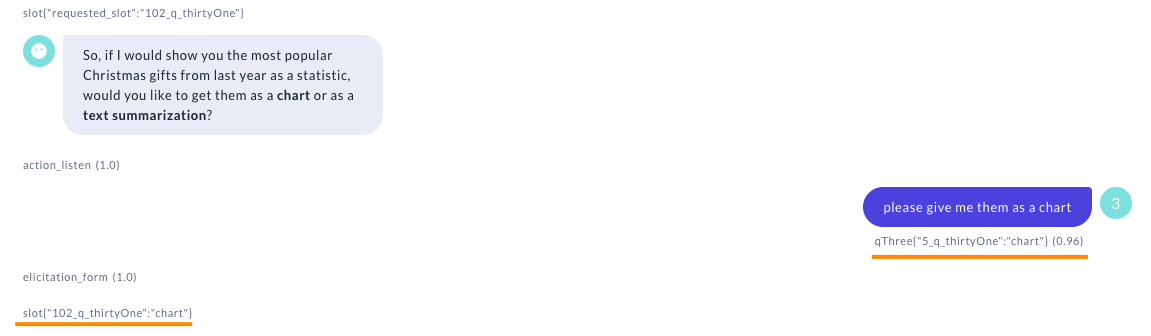
\includegraphics[width=1\linewidth]{images//validateData.png}
   \caption[Rasa X UI (Entwicklersicht): Analyse der gespeicherten Chatgespräche] {Rasa X UI (Entwicklersicht): Analyse der gespeicherten Chatgespräche}
  \label{fig:intentvalidation}
  \end{figure} 

Bei der Frage \glqq would you like to get them as a chart or as a text summarization?\grqq{}
erwartet der Slot des Bots entweder die Entity \textit{chart} oder die Entity \textit{text summarization}. Sofern dieser Slot nicht mit einem von diesen beiden 
Entities gefüllt wird, wird die nächste Frage nicht gestellt. Die rechte orange Markierung in der Abbildung zeigt, dass die Entity \textit{chart}
erkannt wurde. Die linke orange Markierung in der Abbildung stellt die erfolgreiche Speicherung der Entity \textit{chart} für den Slot dar.
\textit{Chart} kennzeichnet die FS-Dimension visuell. Also erhöht sich die Tendenz zum visuellen Lernstil. Auf dieser Weise kann die 
komplette Lernstilklassifikation nachvollzogen werden. \\
Als Nachteil von Rasa X ist zu nennen, dass sich das Profilbild des Avatars nicht einstellen lässt. Zudem wird dem Nutzer 
beim Drücken eines Buttons der Payload, welcher hinter dem Button steckt, angezeigt. Die Abbildung \ref{fig:ButtonID} stellt ein Beispiel dar.
\begin{figure}[H]
    \centering
    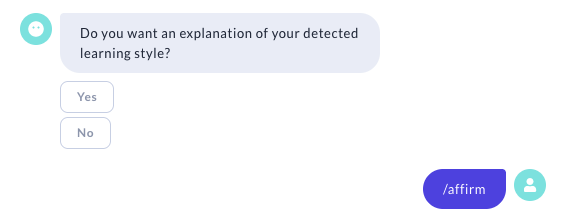
\includegraphics[width=0.6\linewidth]{images//buttonID.png}
   \caption[Rasa X UI: Button-Payload] {Rasa X UI: Button-Payload}
  \label{fig:ButtonID}
  \end{figure} 

Sofern der Nutzer auf den Button 
\glqq yes\grqq{} klickt, wird ihm der payload \glqq /affirm\grqq{} angezeigt. Dies könnte den Nutzer verwirren.
%Übertragung auf DialogFlow
Bezüglich der Übertragung der Trainingsdaten von Rasa zu Google DialogFlow gibt es keine automatisierte Möglichkeit.
Dennoch könnten die Intents und Trainingsdaten in der nlu.yml Datei eingesehen werden und manuell zu Google DialogFlow übertragen werden.

%Prototyp
Der Prototyp befindet sich noch auf Testbasis, daher wurde für die Umfrage (n=25) ein betreutes Experiment vorgesehen, um 
auch gerade zu Anfang gewissenhafte Daten von den Probanden zu erhalten. Das Gewinnen von Studienteilnehmern war aufgrund des 
großen Studienumfangs (Dauer $\geq$ 30 Minuten) schwer. Zudem ist die Umfrage als nicht repräsentativ anzusehen.
Hier bestünde die Möglichkeit, die Umfrage in Vorlesungsveranstaltungen zu integrieren oder Schulen zu besuchen,
um eine größere Anzahl an Teilnehmern zu rekrutieren. 
Dadurch, dass die Befragten wenig Erfahrung mit Chatbots aufwiesen, bestand das Risiko, dass dies die Beantwortung
beeinflusst hat. Außerdem basieren die Ergebnisse der Umfrage zur Beantwortung von RQ1 und RQ2 auf subjektiven Antworten. 
Um der Subjektivität entgegenzuwirken, besteht die Möglichkeit,
die Probanden vor der Interaktion mit Vicky den originalen ILS-Fragebogen nach Felder und Soloman (1991) 
ausfüllen zu lassen, um dann die Lernstilergebnisse aus dem ILS-Fragebogen und den beiden Interaktionen mit Vicky zu vergleichen. 
Bei der Interpretation von RQ2 sollte zusätzlich bedacht werden, dass  
die Trainingsdaten nach jedem Teilnehmer angepasst wurden. Dies könnte die Wahrnehmung der letzteren Teilnehmer beeinflusst haben, da 
sie mit einem robusteren Prototyp interagiert haben. Das unterschiedliche Wahrnehmungsvermögen der Teilnehmer könnte somit RQ2 beeinflusst haben. 
Für eine Lernstilklassifikation nach dem Dialog mit Vicky (1. Interaktion) darf dieser Dialog nicht unterbrochen werden, da die 
Fragen im Dialog bereits auf den 17 reduzierten ILS-Fragen von Latham (2011) basieren (vgl. Kapitel \ref{VorstellungPrototyp}). Inwiefern sich eine weitere Reduktion der Fragen
oder ein Überspringen einer Frage im Dialog auf das Ergebnis auswirkt, kann in Folgearbeiten untersucht werden.

Für die persönliche Ansprache im Chatgespräch war die Identifikation des Namens wichtig.
Aufgrund der Vielfalt an Namen wurde eine große Anzahl an Trainingsdaten verwendet. 
Der Nachteil dabei ist, dass Wörter, die falsch geschrieben wurden, 
manchmal als Name identifiziert wurden. Zum Beispiel wurde anstatt \glqq I learn\grqq{} -
\glqq I lern\grqq{} geschrieben. Vicky hat dann \textit{lern} als Namen angesehen. 
Ein Grund dafür kann sein, dass die Struktur der Trainingsdaten zur Namensidentifikation nur 
einzelne Namen enthalten und somit orientierte sich das Wort \textit{lern} zum Intent \textit{GiveName}, 
da zusätzlich die 
Anzahl an Trainingsdaten des Intents \textit{GiveName} 
deutlich höher ausfiel als die Trainingsdaten zu den anderen Intents.
Allerdings war dies wichtig, damit der Lernende nicht  
\glqq My name is Paul\grqq{} oder \glqq I´m Paul\grqq{}, sondern nur \glqq Paul\grqq{} auf die 
Frage \glqq What´s your name?\grqq{} schreiben konnte. Eine andere Limitation weist die Nutzung der Verneinung auf. 
Um zu umgehen, dass ein Lernender zum Beispiel bei der Frage zur Lernstilklassifikation \glqq Did you memorize it like to get 
a picture or words?\grqq{} nicht mit \glqq I didn´t get it by a picture\grqq{} antwortet und damit nicht eindeutig klarstellt, ob er seine 
Erinnerung anhand von Wörtern hervorruft, untersagt Vicky allgemein Verneinungen. Dies diente dazu, dass die Lernstilidentifikation von Vicky 
nicht auf missverständlichen Antworten basiert.
Ferner kann die Smalltalk-Funktion erweitert werden. Dem Lernenden könnte angeboten werden, den Dialog oder das Quiz-Spiel 
komplett zu unterbrechen und in einen anderen Gesprächsmodus zu wechseln. Außerdem könnte in der Weiterentwicklung
auf weitere und tiefere Rückfragen reagiert werden, um Unklarheiten zu beseitigen und eine höhere Transparenz aufzuweisen. 
Dazu eignen sich weitere Studien, in denen die Probanden nach Unklarheiten und gerne gestellten Rückfragen befragt werden.

Das Quiz-Spiel bietet viele Möglichkeiten für weitere Forschungsarbeiten.
Die Quiz-Fragen basieren auf Knobelaufgaben sowie auf Fragen zum Allgemeinwissen, da allgemein Lernende als Zielgruppe betrachtet wurden. 
Einige Quiz-Fragen wurden als zu mathematisch empfunden. Somit sollten die Quiz-Fragen an die Personengruppen 
angepasst werden. Entweder werden Quiz-Fragen je nach Studiengang gestellt oder der Lernende wird nach seinen Interessen gefragt, die  
dann das Themengebiet für die Quiz-Fragen darstellen, beispielsweise Fragen zur Politik oder Medizin.
Des Weiteren können Spielmechaniken  in das Quiz-Spiel integriert werden. Beispiele 
möglicher Spielmechaniken für das Quiz-Spiel sind: Punktesysteme, Abzeichen, Ranglisten oder Level. 
Zudem weisen diese ein Potenzial auf, individuelle Bedürfnisse und Motive zu aktivieren. \parencite[276]{Blohm.2013} \\
Ferner können die Vorschläge der Probanden zu den weiteren Funktionalitäten eines virtuellen Begleiters und 
der negativ empfundenen Aspekten sowie der Weiterentwicklung der Charaktereigenschaften von Vicky für eine menschenähnlichere Wahrnehmung
(vgl. Kapitel \ref{Kapitel5.2}) in zukünftigen Forschungsarbeiten untersucht werden.

Abschließend konnte durch die Nutzung eines Level-1-Artefakts neues Wissen und neue Erfahrungen hinsichtlich der Möglichkeit 
einer Lernstilklassifikation des Lernenden
sowohl durch eine dialogbasierte Interaktion als auch durch ein Quiz-Spiel zwischen einem CA 
und einem Lernenden in natürlicher Sprache sowie der Einfluss auf die Lernmotivation des Lernenden 
gesammelt werden. Dies trägt dazu bei, die aufgedeckte Forschungslücke zu schmälern.


